\newpage
\section{最大转矩电流比控制技术MTPA}

\subsection{MTPA基本原理}
根据\eqref{eq:同步坐标系下电磁转矩表达式（一般形式）}，对于内置式永磁同步电机IPMSM，
电磁转矩由两部分组成：
\begin{equation*}
    T_{\mathrm{e}}=\cfrac{3}{2}p\psi_{\mathrm{m}}i_{\mathrm{q}}+
    \cfrac{3}{2}pi_{\mathrm{q}}(L_{\mathrm{d}}-L_{\mathrm{q}})i_{\mathrm{d}}
\end{equation*}

其中\(\cfrac{3}{2}p\psi_{\mathrm{m}}i_{\mathrm{q}}\)是线性项，且磁场来源于永磁体磁链，
称为永磁转矩。而\(\cfrac{3}{2}pi_{\mathrm{q}}(L_{\mathrm{d}}-L_{\mathrm{q}})i_{\mathrm{d}}\)是
非线性项，且磁场来源于D轴电流构造，称为磁阻转矩。

在前文的经典FOC控制设计中，让\(i_{\mathrm{d}}^*=0\)来让电机模型尽可能被近似为线性模型，
使得磁阻转矩近似为零。实际上，对于IPMSM有\(L_{\mathrm{d}}-L_{\mathrm{q}}<0\)（忽略磁路饱和时
可近似视为常量），若能够让\(i_{\mathrm{d}}<0\)，则磁阻转矩
\(\cfrac{3}{2}pi_{\mathrm{q}}(L_{\mathrm{d}}-L_{\mathrm{q}})i_{\mathrm{d}}\)在
\(i_{\mathrm{q}}>0\)时为正，产生正的磁阻转矩；而在\(i_{\mathrm{q}}<0\)时为负，产生负的磁阻转矩，此时
磁阻转矩自发根据Q轴电流的正负号调整方向，保持与永磁转矩同号叠加增大
，从而在不增大电流幅值的前提下增大总转矩。因此，
最大转矩电流比控制技术（Maximum Torque Per Ampere，MTPA）应运而生，旨在通过调整D轴电流、激发
磁阻转矩，实现用最小的电流有效值换取最大的电磁转矩。

MTPA首先需要建立最小化电流的目标函数。对于永磁同步电机，在特定负载下稳定运行在特定速度时，
三相电流与电角度满足：
\begin{equation*}
    \begin{cases}
        i_{\mathrm{A}}=\sqrt{2}I\cos(\theta_{\mathrm{e}}+\cfrac{\pi}{2}+\gamma)\\
        i_{\mathrm{B}}=\sqrt{2}I\cos(\theta_{\mathrm{e}}+\cfrac{\pi}{2}+\gamma-\cfrac{2\pi}{3})\\
        i_{\mathrm{C}}=\sqrt{2}I\cos(\theta_{\mathrm{e}}+\cfrac{\pi}{2}+\gamma+\cfrac{2\pi}{3})
    \end{cases}
\end{equation*}

其中\(\sqrt{2}I\)表示单相电流的幅值，对应的单相电流有效值就是\(I\)。而角度\(\gamma\)称为
电流超前角，定义为合成电流矢量超前q轴的角度。在经典FOC中使得\(i_{\mathrm{d}}^*=0\)，
对应电流超前角\(\gamma=0°\)。在坐标系中的关系如下图所示（定义逆时针旋转为正，也是角度
的超前方向）：
\begin{figure}[H]
    \centering
    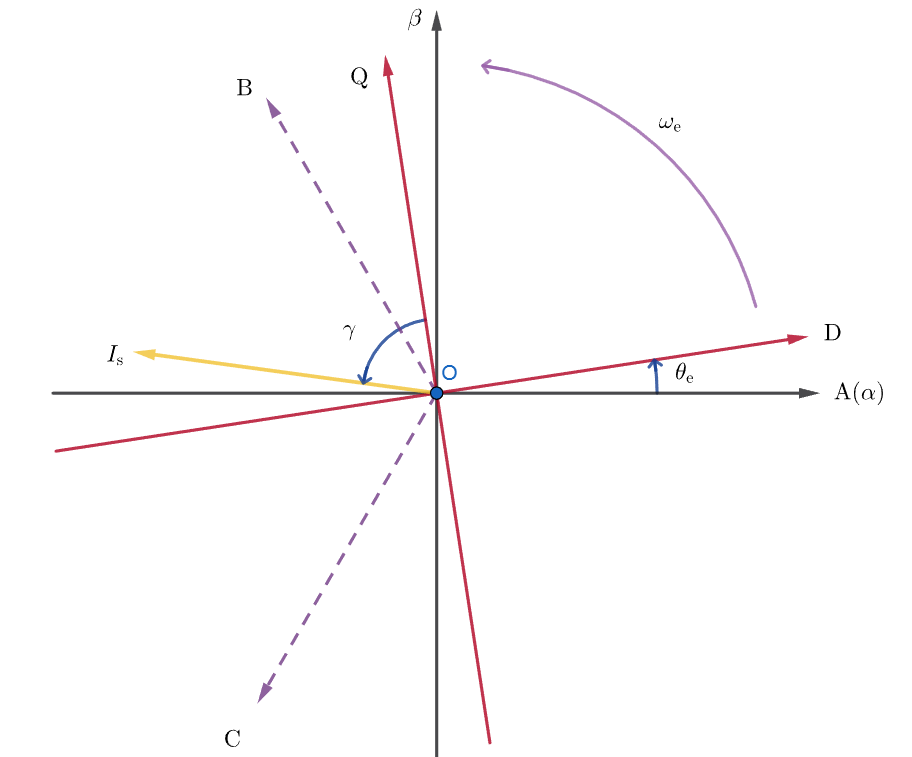
\includegraphics[width=0.6\textwidth]
    {图片/电流超前角定义.png}
    \caption{电流超前角定义}
    \label{fig:电流超前角定义}
\end{figure}

根据克拉克变换\eqref{eq:克拉克变换}
可得：
\begin{equation*}
    \begin{cases}
        i_{\mathrm{\alpha}}=\cfrac{2}{3}i_{\mathrm{A}}-\cfrac{1}{3}i_{\mathrm{B}}-\cfrac{1}{3}i_{\mathrm{C}}
        =\sqrt{2}I\cos(\theta_{\mathrm{e}}+\cfrac{\pi}{2}+\gamma)\\
        i_{\mathrm{\beta}}=\cfrac{\sqrt{3}}{3}i_{\mathrm{B}}-\cfrac{\sqrt{3}}{3}i_{\mathrm{C}}=
        \sqrt{2}I\sin(\theta_{\mathrm{e}}+\cfrac{\pi}{2}+\gamma)
    \end{cases}
\end{equation*}

进一步根据\eqref{eq:帕克变换}可得：
\begin{equation}
    \begin{cases}
        i_{\mathrm{d}}=\cos\theta_{\mathrm{e}}i_{\mathrm{\alpha}}+\sin\theta_{\mathrm{e}}i_{\mathrm{\beta}}
        =-\sqrt{2}I\sin\gamma\\
        i_{\mathrm{q}}=-\sin\theta_{\mathrm{e}}i_{\mathrm{\alpha}}+\cos\theta_{\mathrm{e}}i_{\mathrm{\beta}}
        =\sqrt{2}I\cos\gamma
    \end{cases}
    \label{eq:DQ电流超前角关系}
\end{equation}

上式给出了DQ电流与电流超前角\(\gamma\)的定量关系。并且
当\(0°<\gamma<180°\)时\(i_{\mathrm{d}}<0\)，电流矢量由q轴向-d轴方向偏移，进入MTPA工作区。

根据上式可知，最小化三相电流有效值\(I\)与最小化DQ电流合成矢量的模长
\(\sqrt{i_{\mathrm{d}}^2+i_{\mathrm{q}}^2}=\sqrt{2}I\)的条件是一致的，而
系数\(\cfrac{\sqrt{2}}{2}\)为常数，不影响取极值条件。为表述方便，记
\begin{equation*}
    I_{\mathrm{s}}=\sqrt{i_{\mathrm{d}}^2+i_{\mathrm{q}}^2}=\sqrt{2}I
\end{equation*}
MTPA的优化目标即为最小化\(I_{\mathrm{s}}\)，即最小化相电流的峰值，而此时相电流有效值也会最低。
